\documentclass[11pt,journal,draftclsnofoot,onecolumn,twoside,letterpaper]{IEEEtran}

\usepackage{indentfirst}
\usepackage{cite}
\usepackage{subfigure}
\usepackage{amssymb}
\usepackage{amsmath}
\usepackage{amsthm}
\usepackage{multicol}
\usepackage{amsfonts}
\usepackage{geometry}
\usepackage{times}
\usepackage[dvips]{graphicx}
\usepackage{fancybox}
\usepackage{url}
\usepackage{bm}
\usepackage{dsfont}
\usepackage{stfloats}
\usepackage{comment}
\usepackage[normalem]{ulem}
%\usepackage[right]{showlabels}
\usepackage[usenames]{color}

\newcommand{\figw}{1.0\linewidth}
\newcommand{\figwless}{0.6\linewidth}
\newcommand{\figws}{0.45\linewidth}
\newcommand{\ben}{\begin{enumerate}}
\newcommand{\een}{\end{enumerate}}
\newcommand{\be}{\begin{equation}}
\newcommand{\ee}{\end{equation}}
\newcommand{\bea}{\begin{eqnarray}}
\newcommand{\eea}{\end{eqnarray}}
\newcommand{\bc}{\begin{cases}}
\newcommand{\ec}{\end{cases}}
\newcommand{\bi}{\begin{itemize}}
\newcommand{\ei}{\end{itemize}}
\newcommand{\e}{\item}
\newcommand{\eq}[1]{(\ref{#1})}
\newcommand{\deeff}{\,\mathrm{d}\;\!\!f}
\newcommand{\de}[1]{\,\mathrm{d}#1}
\newcommand{\meas}[1]{\,\,\!\mathrm{#1}}
\newcommand{\pc}[1]{\textbf{(PC: #1)}}
\newcommand{\dc}[1]{\textbf{(DC: #1)}}
\newcommand{\vup}{\vspace{-1mm}}
\newcommand{\back}{\!\!\!\!\!}
\newcommand{\bre}{\begin{bf}\begin{color}{BrickRed} }
\newcommand{\ere}{\end{color} \end{bf}}
\newcommand{\RM}[1]{\begin{color}{BrickRed} (RM: #1) \end{color}}
\newcommand{\MP}[1]{\begin{color}{NavyBlue} (MP: #1) \end{color}}
\newcommand{\PC}[1]{\begin{color}{ForestGreen} (PC: #1) \end{color}}

\theoremstyle{definition} \newtheorem{definition}[]{Definition}

\theoremstyle{theorem} \newtheorem{theorem}[]{Theorem}


\DeclareMathOperator{\Var}{Var}
\DeclareMathOperator{\VEC}{vec}
\DeclareMathOperator{\diag}{diag}
\DeclareMathOperator*{\argmax}{arg max}

\def\C(#1){{\cal #1}} % calligraphic style
\def\B(#1){\hbox{\boldmath$#1$}} % bold style




\newcounter{mytempeqn}

%\baselineskip 24pt
\renewcommand{\baselinestretch}{1.75}

%\setlength\floatsep{0.98\baselineskip}
%\setlength\textfloatsep{0.98\baselineskip}

\geometry{verbose,letterpaper,tmargin=1.05in,bmargin=1.0in,lmargin=0.75in,rmargin=0.75in}

% *** GRAPHICS RELATED PACKAGES ***
%
\ifCLASSINFOpdf
  % \usepackage[pdftex]{graphicx}
  % declare the path(s) where your graphic files are
  % \graphicspath{{../pdf/}{../jpeg/}}
  % and their extensions so you won't have to specify these with
  % every instance of \includegraphics
  % \DeclareGraphicsExtensions{.pdf,.jpeg,.png}
\else
  % or other class option (dvipsone, dvipdf, if not using dvips). graphicx
  % will default to the driver specified in the system graphics.cfg if no
  % driver is specified.
  % \usepackage[dvips]{graphicx}
  % declare the path(s) where your graphic files are
  % \graphicspath{{../eps/}}
  % and their extensions so you won't have to specify these with
  % every instance of \includegraphics
  % \DeclareGraphicsExtensions{.eps}
\fi


% correct bad hyphenation here
\hyphenation{op-tical net-works semi-conduc-tor}

\IEEEoverridecommandlockouts

\begin{document}

\pagestyle{empty}

\begin{Large} \noindent {\bf Department of Information Engineering (DEI), University of Padua}\\ \end{Large}
\begin{large} {Meeting minutes} \end{large}

\vspace{0.8cm}

\noindent {\it Meeting: } $13^{th}$ meeting of the SIGNET Underwater Group.\\
{\it Date of the meeting: } Tue $11^{th}$ of September $2012$\\
{\it Present: } Giovanni Toso (CFR), Federico Favaro (CFR), Matteo Petrani (CFR), Paolo Casari (CFR and DEI, UniPD), Ivano Calabrese (CFR)\\

\vspace{0.5cm}

\begin{tabular}{p{0.9\columnwidth}}
 \hline \\
\end{tabular}


\noindent {\bf Agenda item A:} Look-up tables for the Physical Layer (RACUN project).\\
{\bf Presenters:} Paolo Casari\\

{\bf Discussion:}\\

\textbf{The following material is taken from the minutes of meeting no. 10, and is re-arranged and partly integrated here in order to re-frame the discussion.}

From the point of view of the network simulations, having RACUN's PHY layer model basically means to have the Packet Error Rate (PER) of several modulation schemes as a function of some scenario and transmitter-related parameters. The PER in the form of a look up table (LUT).

The LUT for RACUN:
\begin{itemize}
  \item provides the PER;
  \item as a function of the following parameters
    \begin{itemize}
      \item Area of measurement
      \item Link type (e.g., bottom-bottom, bottom-surface, mobile-bottom, etc.)
      \item Modulation Scheme (Several combinations of packet size and data rate, final number not completely known probably $\sim$25)
      \item SNR
    \end{itemize}
\end{itemize}

One PER estimate for each parameter combination will be provided.

The question is now how to import and use this LUT in NS-Miracle.

We have three levels of actions: 1) preparing the data so that it can be loaded in NS-Miracle as C++ code; 2) prepare the module in NS-Miracle to exploit the LUT (exported in C++); 3) decide the mechanism to retrieve, from the LUT (exported in C++), the actual PER to use in the simulations.

As opposed to what we initially decided (re-parse data, modify dumb wireless channel, build ordered PER list and load it into the modified dumb wireless channel), the process has changed slightly. What we will need to do is the following:
\begin{enumerate}
 \item for each scenario (Area, Modulation scheme) convert the .mat structure that will be provided by Paul van Walree into a \textbf{binary} file, and which can be accessed to using offsets to retrieve the desired PER values as a function of (SNR and link types). The output of the parser will be a C++ code with all the commands required to create this binary file, which will be accessed by NS-Miracle's PHY-level module \RM{Is it already define the actual structure and organization of such binary file? And how to handle/retrieve/use the offsets?} \PC{Not yet, I guess it will be food for thought at the next meeting.}\\
 It has been decided not to set up a large matrix with all values, in order to avoid loading too much data in the RAM.  
 \item once a given scenario (TCL) has been specified, when a transmission take place we know the area, modulation scheme and link type, and we need to compute the SNR; we do so using WOSS's Urick model with a path loss coefficient of $k=1.75$. This will provide the received power, which will be divided by the noise power to yield the SNR. The SNR will be fed to the LUT and the PER will be retrieved \PC{As an answer to Riccardo's comment} via ``nearest neighbor'' interpolation: this means that if the SNR values in the LUT are $\{ -10, -9.5, -9, \ldots , 29.5, 30\}$, and an SNR of $12.2$~dB is computed, then the PER for an SNR of $12$~dB will be retrieved and used.
 \item The noise will be computed according to empirical equations. These equations will be taken from chapter 6 of RACUN deliverable D4.1.1, of WE 4100, on the RACUN server, and will be implemented along with the equations currently used in NS-Miracle. A Matlab version of the noise models can be found on the RACUN web server under RACUN Project $>$ Shared Documents $>$ WE4100 $>$ D412 $>$ Noisemodel.
 \item After the received power has been computed using Urick's model, we have two cases:
	\begin{enumerate}
	 \item \emph{Absence of collisions}: the received power will be divided by the noise power to yield the SNR. The SNR will be fed to the LUT and the PER will be retrieved. 
	 \item \emph{Presence of collisions}: see next discussion point.
	\end{enumerate}
\end{enumerate} 

So far we received only one Matlab data file from Paul van Walree. More are coming after Paolo's meeting with Paul at UCOMMS in Sestri Levante.

The LUTs containing the PER in the presence of collisions are not ready yet.

{\bf Conclusions:}\\
After the MAT files have been received from Paul, start the implementation of the modules.
\  \\

\noindent {\bf Agenda item B:} RACUN PER lookup tables in the presence of collisions.\\
{\bf Presenters:} Paolo Casari\\
{\bf Discussion:}\\

The presence of collisions and their impact on packet reception will be modeled using physical layer simulations. Some LUTs will be generated, akin to those provided for PER vs.~SNR. These LUTs will provide the PER as a function of the Area, Modulation scheme, Link type, and two more parameters: the overlap $\omega$ and the Signal-to-Interference Ratio (SIR) $\gamma_I$. 
With reference to Fig.~\ref{fig:coll1}, these two parameters are defined as $\omega = \frac{t_A^2 - t_B^1}{t_A^2-t_A^1}$, and $\gamma_I = \frac{P_A}{P_B}$.

\begin{figure}[h!]
  \begin{minipage}[t]{0.48\columnwidth}
	\centering
	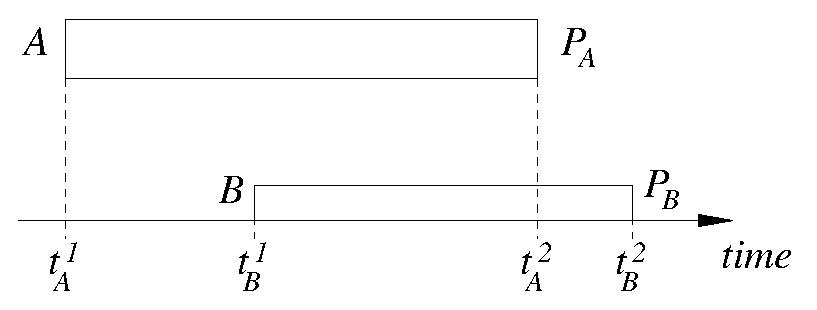
\includegraphics[width=\linewidth]{figures/collision_simple.eps}
	\caption{Reference timings for the definition of $\omega$ and $\gamma_I$ in the case of constant interference.}
	\label{fig:coll1}
  \end{minipage}
  \hfill
  \begin{minipage}[t]{0.48\linewidth}
	\centering
	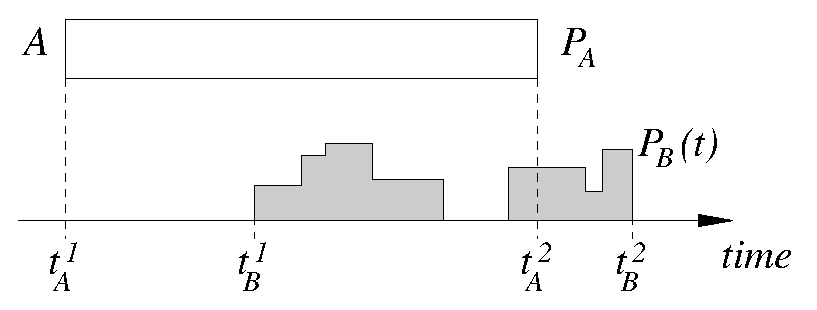
\includegraphics[width=\linewidth]{figures/collision.eps}
	\caption{Reference timings for the definition of $\omega$ and $\gamma_I$ in the case of time-varying interference.}
	\label{fig:coll2}
  \end{minipage}
\end{figure}

The question now is how we should behave in a more general interference scenario such as that depicted in Fig.~\ref{fig:coll2}, where the power of the interference affecting packet A varies over time. In this case, we have agreed with Roald Otnes and Paul van Walree to compute the overlap as $\omega = \frac{t_A^2 - t_B^1}{t_A^2-t_A^1}$ regardless of the fact that there may be discontinuities in the interfering power between $t_B^1$ and $t_A^2$. The interfering power will then be averaged over the $[t_B^1,t_A^2]$ interval as $\bar{P}_B = \int_{t_B^1}^{t_A^2} P_B (t) \de{t}$, and we will calculate $\gamma_I = \frac{P_A}{\bar{P}_B}$.
Although approximated, this model is much better than what is currently considered in most simulators, which treat all interference as Gaussian noise.

NOTES:\\
(1) there are cases where $\omega = 1$, e.g., when a reception is going on (e.g., packet A of Fig.~\ref{fig:coll1}), a long interferer (e.g., packet B of Fig.~\ref{fig:coll1}) starts before the end of A, NS-Miracle does not sync on B, and another packet (say, C) starts just after the end of A's reception).\\
(2) we assume that in such cases as the one in Fig.~\ref{fig:coll1}, the receiver will never switch from the reception of A to the reception of B, but it will proceed directly to the reception of C.


{\bf Conclusions:}\\
Federico Favaro confirmed that this is very likely possible and will double check. Confirmation to be provided by Friday Sep 21, 2012.

Paul van Walree will provide LUTs where the PER for packet A is given as a function of Area, Modulation Scheme, Link type, and then $\omega$ and $\gamma_I$. Delivery time still unknown.
\  \\



\noindent {\bf Agenda item C:} Integration of NS-Miracle within the SAAB modem\\
{\bf Presenter:} Paolo Casari\\
{\bf Discussion:} \\

At SAAB, the main people in charge of the integration of NS-Miracle are Jakob Lingren and Johan Carlstr\"{o}m. They have installed VMWare on the computer that implements the software for the SAAB modem and carries the RACUN framework (PHY, NET, APP). They have been testing UDP comms between the two machines (the outcome of this test is unknown) \RM{using which code?} \PC{I asked, apparently no code. Updates to come at the meeting}.

The idea is to help them perform the integration of NS-Miracle into the framework. Paolo expects them to call us there when this UDP communications is in fact working.

A proposal we made to them is to make and send them an image with all software already installed, and exported for use with VMWare. No positive or negative answer received yet. An exchange of emails is going on between me, Matteo and the SAAB guys.

{\bf Conclusions:}\\
At this time, Giovanni should have prepared the image for Matteo Petrani to install all software required to run the RACUN demo. Matteo Petrani is to continue the discussion with the SAAB guys.
\  \\




\noindent {\bf Agenda item D:} RACUN demo on our SVN repository.\\
{\bf Presenter:} Paolo Casari \\
{\bf Discussion:} \\

It has been decided to give access to our svn server (https://telecom.dei.unipd.it/tlcrepos/underwater/RACUN/) to all RACUN members that are interested in downloading the code for the RACUN demo and in contributing to the experiments.

{\bf Conclusions:} \\
Paolo collected interests in being given access to the svn and sent an email to Simone Friso. The people who expressed interest are:
\begin{itemize}
 \item    Roald Otnes  -  Roald.Otnes@ffi.no
 \item    Jan Nilsson  -  jan.nilsson@foi.se
 \item    Jakob Lindgren  -  jakob.lindgren@saabgroup.com
 \item    Michael Goetz  -  goetzm@wimas.de
 \item    Joerg Kalwa  -  joerg.kalwa@atlas-elektronik.com
 \item    Henry Dol  -  henry.dol@tno.nl
 \item    Sabrina Schreiber  -  Sabrina.Schreiber@l-3com.com
 \item    Johan Carlstr\"{o}m  -  johan.carlstrom@saabgroup.com
 \item    Helge Buen  -  helge.buen@ffi.no
 \item    Bastien Lyonnet  -  bastien.lyonnet@tno.nl
 \item    Hendrik Schelenz  -  Hendrik.Schelenz@atlas-elektronik.com
 \item    Ivor Nissen  -  IvorNissen@bwb.org
\end{itemize}
\  \\


\noindent {\bf Agenda item E:} How do we proceed towards RACUN's ST2? (April 2012).\\
{\bf Presenter:} Paolo Casari \\
{\bf Discussion:} \\

Several deadlines have been fixed and are outlined in Table~\ref{tab:deadlines_ST2} \RM{What about the issue of having two separate networks or two parts connected by a gateway?} \PC{I told many people separately that we should not address two separate networks using separate PHYs in the same band, but rather test them independently, and use FMT as the only common PHY that will enable a large-size network. It seems everyone agrees, but since we don't even have FMT in the SAAB modem, it is too early to raise the issue now}.

In addition to the tasks below, there is one more task for which there is no clear deadline: we should prepare a standardized way to perform event logging during the tests. Ivor Nissen sent an email that proposes to format the data related to several events (e.g., parcel generation, parcel reception with this and that contents at this time, et.c) in a standardized csv format, so that we can use some already prepared scripts to convert the csv into a SQL database for easy recovery.
Paolo will forward the related email, to be read for comments by all the people present at the meeting, plus Riccardo.
\RM{I have read the mail of Ivor and I believe that they have done a good thing. It would be nice and useful to have a common way of printing debug/log messages. In particular, from what I understand, in the RACUN framework is already present a function called Log that allows one to print log messages according to the format proposed by Ivor, that, in my opinion, is fine. So far in NS-Miracle we do not have a standardized way to print debug and log messages: each module-developer adopted different solution according to his/her own tastes. What we should do, then, is: 1) understand how to call/use the Log function of RACUN within the NS-Miracle framework that is running on a parallel process (it may be possible for instance just doing a cut and paste of such function in one or more of our modules and declare it as static. However, I believe this will work only for messages to print in cout; not sure about how to print in the same log file for all the RACUN framework contained in a node); 2) replace, for each 
module to be put in RACUN\_NET\_MIRACLE, all the debug/log message according to the Log function of above.}

\begin{table}[t]
  \centering
  \caption{Deadlines from now to the RACUN Sea Trial \# 2.}
  \label{tab:deadlines_ST2}
  \begin{tabular}{|r|p{14cm}|}
    \hline
    Deadline  &  Objective \\
    \hline \hline
    17/09/2012  &  Node provider shall send a list of command (GUWAL) which can be processed by the APP \\
    30/09/2012  &  TNO distributes ST2 Scenario / Storyboard draft \\
    30/09/2012  &  DESERT underwater runs on the SAAB modems, compatibility of ELAC software with NS-Miracle is                                          		verified \\
    15/10/2012  &  TCL scripting starts after Scenario description (triggered by Uni Padova)\\
    18/10/2012  &  Trial Detailing Meeting (week 42) \RM{how? where?} \\
    30/11/1012  &  All Software prepared (protocols, bitstream mappings, TCL scripts for ALL experiments) \\
    31/12/2012  &  All code is working in NS Miracle (on PC Demo working at participating partners, experiment 			management tools working) \\
    15/01/2013  &  Integration dry test \\
    15/02/2013  &  Pre-Factory Adaptation Test (Pre-FAT) in water in Kiel (week 7/8 of 2013) \\
    06/03/2013  &  HYPPR 5 meeting, Den Haag \\
    08/04/2013  &  FAT in Den Helder, The Netherlands \\
    10/04/2012  &  RACUN ST2 are held in Den Helder (total duration: 2 weeks, expected effective operational 			hours: 24-48)\\
    \hline
  \end{tabular}
\end{table}



{\bf Conclusions:} \\
There are no substantial delays in the work to be reported so far.

Paolo will forward the email related to data logging, to be read for comments by all the people present at the meeting, plus Riccardo.



\newpage

\noindent {\bf Overall conclusions: } 

In the following we summarize the actions points decided up to the above discussions. 

\begin{tabular}{|p{0.05\columnwidth}|p{0.5\columnwidth}|p{0.2\columnwidth}|p{0.15\columnwidth}|}
\hline
{\it Item} & {\it Action Description} & {\it Person responsible} & {\it Deadline (DD/MM/YYYY)}\\
\hline
A1 &  Retrieve PER vs.~SNR LUTs from Paul & Paolo  & 30/09/2012 \\ 
A2 &  Prepare VM to be sent to SAAB & Matteo, Giovanni  &  14/09/2012\\
A3 &  Organize integration meeting with SAAB & Paolo & 21/09/2012 \\
A4 &  Check whether the (overlap+SIR) collision model can be implemented in NS-Miracle & Fede Favaro & 21/09/2012\\
A5 &  Provide access to the RACUN path on the svn server for RACUN members & Paolo & 14/09/2012\\ 
A6 &  Forward proposal for data logging by Ivor Nissen to the group & Paolo & asap \\
\hline
\end{tabular}
\ \\
\ \\
{\bf Verification Points:}
\begin{itemize}
  \item {\bf A1}: Up to Thu Sep 13, 2012, only one example mat file from Paul van Walree is available. Full set of LUTs retrieved on Fri Sep 14, 2012. 
  \item {\bf A2}: VM and HOWTOs ready
  \item {\bf A3}: As of Fri 14, 2012, we received an invitation from SAAB. Follow-up expected by email.
  \item {\bf A4}:
  \item {\bf A5}: List of interested people collected until Tue Sep 11, 2012. Mail sent to Simone Friso on Sep Thu 13, 2012. Accounts created on Fri Sep 14, 2012. Usernames and passwords sent to everyone on Fri Sep 14, 2012.
  \item {\bf A6}: Mail forwarded on Thu Sep 13, 2012.
\end{itemize}


\end{document}
